\documentclass[12pt,a4paper]{article}

\usepackage[margin=2.9cm]{geometry}
\usepackage{graphicx}
\usepackage{titling}
\usepackage{hyperref}
\usepackage{amsmath}
\usepackage{caption}
\usepackage{microtype}
\usepackage{titlesec}
\usepackage{float}
\usepackage{wrapfig}

\graphicspath{{images/}}
\hypersetup{colorlinks=true,urlcolor=blue,citecolor=blue,linkcolor=black}
\captionsetup{font=small,skip=2pt}
\setlength{\droptitle}{-1.5cm}
\setlength{\textfloatsep}{5pt}
\setlength{\floatsep}{5pt}
\setlength{\intextsep}{5pt}
\setlength{\parskip}{0pt}
\setlength{\emergencystretch}{2em}
\titlespacing*{\section}{0pt}{5pt}{2pt}
\titlespacing*{\subsection}{0pt}{4pt}{1pt}

\title{Modern Search Engines: TUE Search}
\author{Lukas Henzler, Nico Henzler, Samuel Scheer, Tuba Aykan}
\date{5 August 2026}

\begin{document}

\maketitle
\vspace{-1.8em}

\section{Introduction}

TUE Search is a focused search engine for English web pages related to Tübingen. It implements crawling, document processing, indexing, retrieval, and result presentation in Python without a dedicated search-engine framework. The main design goal is to combine efficient lexical retrieval with semantic and authority signals while remaining practical on ordinary hardware. Expensive work, such as document encoding, PageRank, and AI-content detection, is therefore performed offline. At query time, the system only filters a limited candidate set, encodes the query, and combines stored signals.

The ranking follows a fast-to-smart funnel. A lightweight TF-IDF-inspired estimate reduces the search space, BM25 selects lexically relevant documents, BERT reranks them by semantic similarity, and PageRank adds an authority signal. Each stage is more expensive but processes fewer documents than the previous one.

\section{System Architecture and Database}

SQLite is the shared storage layer and source of truth for the crawler, indexer, and query processor. It requires no database server but still provides transactions, constraints, aggregation, and persistent state. Figure~\ref{fig:schema} shows the current schema. \texttt{documents} contains URL metadata, crawl state, PageRank, and a reference to stored content. \texttt{terms} and \texttt{postings} form the inverted index; \texttt{links} stores the directed web graph; \texttt{content} stores extracted text, its SimHash, and an AI probability; and \texttt{embeddings} contains neural document vectors.

\begin{figure}[H]
    \centering
    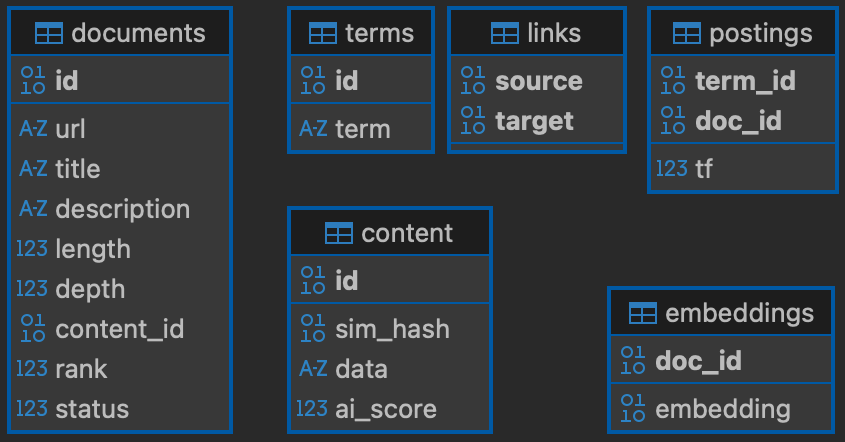
\includegraphics[width=0.78\linewidth]{schema.png}
    \caption{SQLite schema of the current implementation.}
    \label{fig:schema}
\end{figure}

Most tables are \texttt{STRICT} and \texttt{WITHOUT ROWID}; explicit primary keys therefore act as storage keys without an extra hidden identifier. Composite keys prevent duplicate posting and link pairs. URLs are normalised by removing query parameters, fragments, and trailing slashes. A \texttt{UNIQUE} constraint together with \texttt{ON CONFLICT DO NOTHING} safely prevents the same normalised URL from entering the frontier twice, even if several crawler threads discover it at the same time.

The database also performs candidate aggregation before detailed ranking. Embeddings and hashes are stored as binary values rather than text, reducing storage and parsing overhead. Keeping the frontier, content, features, and ranking data together also supports recovery after an interrupted crawl.

\section{Crawler and Document Processing}

The crawler begins with Tübingen-related seed pages and explores links up to the configured depth. Every URL has a status: pending, queued, cached, ready, skipped, or error. Polling changes pending rows to queued rows atomically, so only one worker receives each page. On restart, stale queued and error rows become pending again, while cached pages continue with indexing. This database-backed state makes the crawl restartable without a separate recovery file.

Downloading is I/O-bound, so the crawler uses multiple threads. Responses are streamed in 16 KiB chunks, limited to HTML documents of at most 2 MiB, and retried when appropriate. The crawler sends an identifiable user agent, requests English content, respects \texttt{robots.txt}, and caches parsed robots policies both on disk and in memory. Temporary HTML files separate downloading from indexing and can be removed once their searchable representation is stored.

Beautiful Soup with the \texttt{lxml} parser extracts titles, descriptions, visible text, and outgoing links. Navigation, header, footer, and aside elements are removed because they often contain repeated template text. Useful image alternative text is retained. English-language and Tübingen relevance checks then reject unsuitable pages. These simple rules favour corpus precision, although unusual page layouts or indirect references to Tübingen can reduce recall.

\section{Indexing and Offline Features}

Indexing is CPU-bound and therefore uses processes rather than threads, avoiding Python's Global Interpreter Lock for preprocessing and duplicate detection. The default configuration starts twelve indexer processes, matching the intended processor count of our development machines; \texttt{--indexers} should be used to set the processor count on another machine. A multiprocessing queue connects the crawler threads to these workers, while a small thread forwards progress messages to the terminal.

Documents and queries share the same lexical preprocessing: lower-casing, removal of punctuation-only tokens and English stop words, German umlaut normalisation, and WordNet lemmatisation. We selected lemmatisation because Porter and Snowball stemming often produced overly aggressive forms in our corpus. Term frequencies and document lengths are stored for later BM25 scoring.

The indexer also removes near-duplicate content in two steps. It first creates a 64-bit SimHash from weighted character trigrams. After that SQLite uses Hamming distance to select at most ten close hash candidates, with fewer than five differing bits. Only these candidates receive the more expensive Jaccard-distance comparison over their word sets. Content with a Jaccard distance below 0.02 reuses the existing content record; otherwise its SHA-256 identifier, text, and SimHash are stored. This cascade is faster than comparing every new page with all indexed content and detects duplicates that URL normalisation cannot find.

After crawling PageRank is computed for ten iterations with a damping factor of 0.85 over links between ready documents. Missing document embeddings are calculated with our custom, fine-tuned BERT model that was trained on msmarco-bm25 with 10k steps. Title, description, and content are encoded together and mean-pooled; vectors are stored for reuse. Both operations are offline because the corpus does not change during querying. Finally, the ModernBERT AI detector from AICodexLab assigns each unique content record an AI-generation probability and stores the result in \texttt{content.ai\_score}. This score is an optional transparency feature in the interface and does not affect retrieval ranking. Its reliability is limited because the pretrained detector may not match the domain of crawled websites. The steps that require ML select CUDA, Apple MPS, or CPU depending on availability for better performance.

\section{Retrieval and Ranking}

\begin{wrapfigure}{l}{0.5\linewidth}
    \centering
    \vspace{-0.7em}
    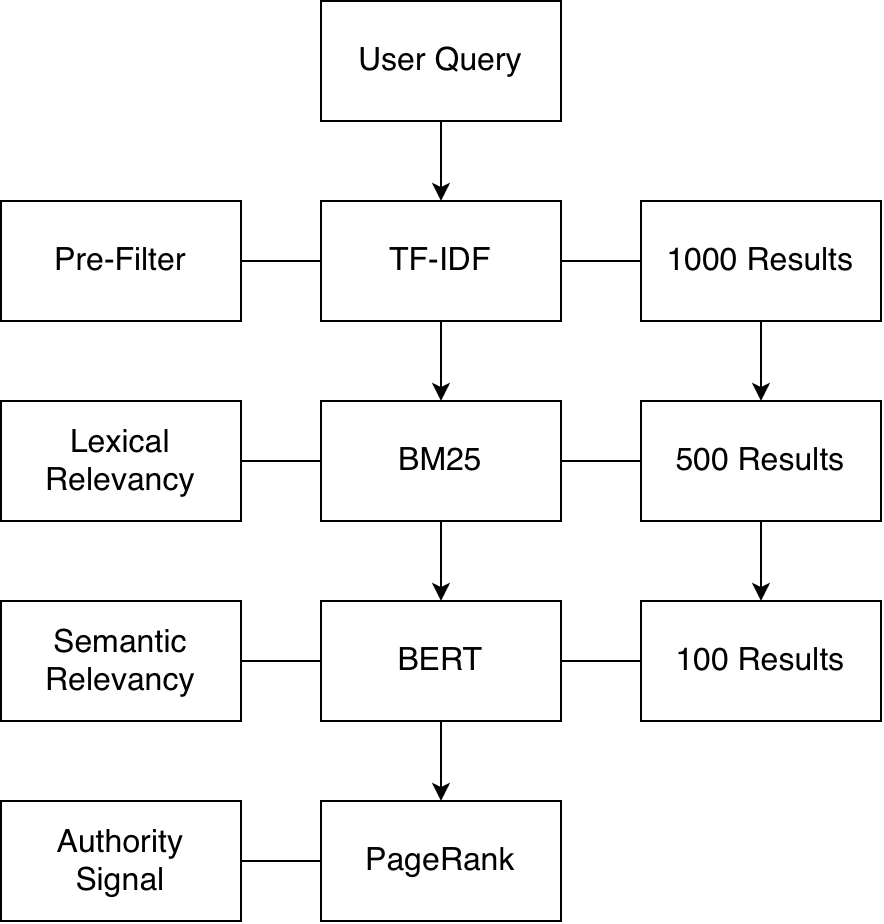
\includegraphics[width=\linewidth]{rankingPipeline.png}
    \captionof{figure}{Fast-to-smart ranking pipeline.}
    \label{fig:pipeline}
\end{wrapfigure}

For an output limit of 100, SQL first keeps at most 1,000 candidates using
\begin{equation}
    S_{\mathrm{pre}}(d,q)=
    \sum_{t\in q\cap d}\mathrm{tf}(t,d)\frac{N}{\mathrm{df}(t)},
    \label{eq:pre}
\end{equation}
where $N$ is the number of ready documents and $\mathrm{df}(t)$ is the document frequency of term $t$. This inexpensive estimate reduces database transfer; it is not the final relevance score.

Our BM25 implementation then applies term saturation and document-length normalisation and keeps the best 500 lexical candidates. BERT encodes the query with the same model used for documents and ranks candidates by cosine similarity. Because document vectors are precomputed, this bi-encoder design requires only one live model encoding. The best 100 semantic candidates receive the final PageRank adjustment.

PageRank is log-transformed and divided by the maximum transformed PageRank in the final candidate set. This puts the authority signal on a controlled scale. The final score is

\begin{equation}
    S_{\mathrm{final}}(d,q)
    =0.7\,S_{\mathrm{BERT}}(d,q)+0.3\,\widehat{PR}(d).
    \label{eq:final}
\end{equation}

Semantic similarity remains dominant, while well-connected pages receive a limited boost. BM25 is intentionally used as a gate rather than added to the final score, avoiding an additional score with a different numerical range. The fixed 70/30 weighting is a reasonable relevance-first choice, but should be tuned on held-out relevance judgements in a larger evaluation.

\section{User Interface}

The interface is built with Textual and remains usable in a graphical or terminal-only environment. Searches run in a background thread, so a loading indicator can remain responsive. Results show a title, URL, and description and can be selected with the keyboard or mouse to open the page. Recent queries can be repeated from the search screen.

\begin{figure}[H]
    \centering
    \begin{minipage}{0.48\linewidth}
        \centering
        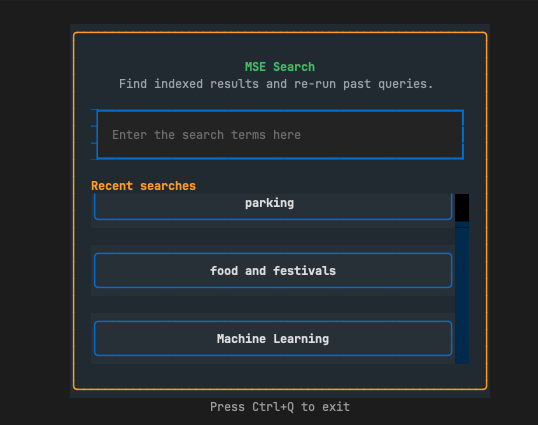
\includegraphics[height=5.5cm,keepaspectratio]{ui_searchInteface.png}
    \end{minipage}\hfill
    \begin{minipage}{0.48\linewidth}
        \centering
        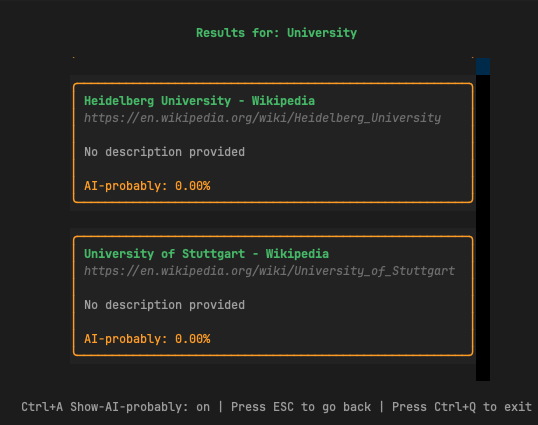
\includegraphics[height=5.5cm,keepaspectratio]{ui_resultsList.png}
    \end{minipage}
    \caption{Search history and query input (left); ranked results with AI probability (right).}
    \label{fig:ui}
\end{figure}

The AI probability is hidden by default because it increases result height and is less reliable than the retrieval score. The user can toggle it with Ctrl+A. Escape returns to the search screen and Ctrl+Q exits from any screen. The footer displays these controls, reducing the need for separate instructions.

\section{Design Trade-offs and Limitations}

The cascade saves computation but creates dependencies: BERT cannot recover a relevant document that the lexical stages exclude. BERT also truncates long pages, and the embeddings are trained on general rather than in-domain data (Tübingen). PageRank measures graph authority rather than factual quality, so its weight is limited to 30\%. Similarly, the language and topic filters favour precision over coverage. Near-duplicate detection uses efficient thresholds but may still merge very similar pages or miss duplicates with substantially changed wording. The AI detector is presented as an optional estimate rather than a verified fact; domain-specific fine-tuning and calibration would be required for stronger claims.

\section{Repository Link}

The final project is available at \url{https://github.com/wiretux/MSE-Project}.

\begin{thebibliography}{3}\small
\bibitem{devlin2019bert} J. Devlin et al. \emph{BERT: Pre-training of Deep Bidirectional Transformers for Language Understanding}. NAACL-HLT, 2019.
\bibitem{page1999pagerank} L. Page et al. \emph{The PageRank Citation Ranking: Bringing Order to the Web}. Stanford InfoLab, 1999.
\bibitem{robertson2009bm25} S. Robertson and H. Zaragoza. \emph{The Probabilistic Relevance Framework: BM25 and Beyond}. Foundations and Trends in Information Retrieval, 2009.
\end{thebibliography}

\end{document}
